\chapter*{PHỤ LỤC}
\addcontentsline{toc}{chapter}{PHỤ LỤC}
\setcounter{figure}{0}
\setcounter{table}{0}
\renewcommand{\thefigure}{A.\arabic{figure}}
\renewcommand{\thetable}{A.\arabic{table}}
    \section{Các linh kiện điện}
        \subsection[Cảm biến hồng ngoại TCRT5000]{Cảm biến hồng ngoại TCRT5000\footnote{Tài liệu tham khảo: \cite{vishay_tcrt5000_1}, trang 4}}
            \begin{figure}[H]
                \centering
                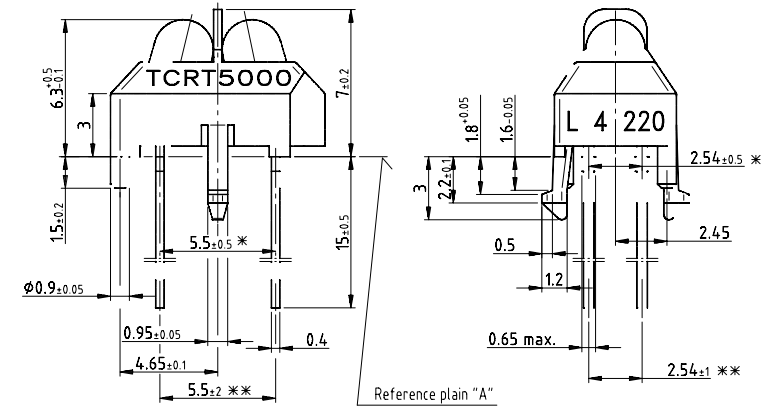
\includegraphics[width=0.88\textwidth]{pictures/appendix/app_p1_TCRT5000Dimensions1.png}
                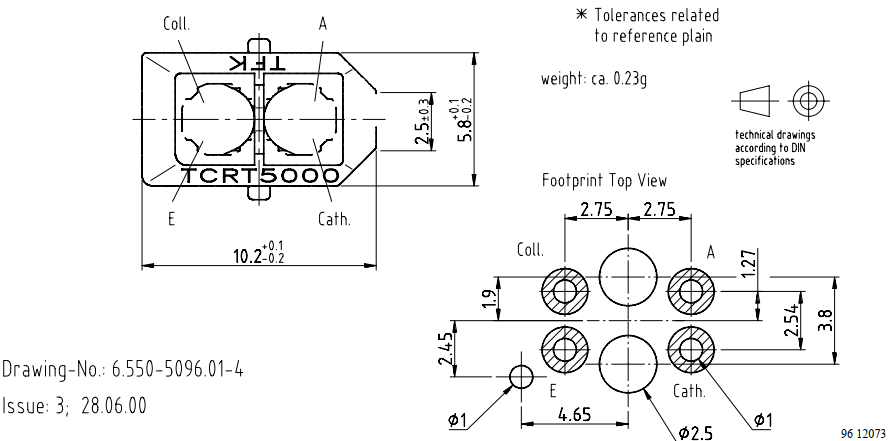
\includegraphics[width=0.88\textwidth]{pictures/appendix/app_p2_TCRT5000Dimensions2.png}
                \caption{Cảm kích thước của cảm biến hồng ngoại TCRT5000}
                \label{fig:TCRT5000}
            \end{figure}
        \subsection[Tụ điện và cuộn cảm cho mạch hạ áp]{Tụ điện và cuộn cảm cho mạch hạ áp\footnote{Tài liệu tham khảo: \cite{lm2596}, trang 25}}
            \begin{figure}[H]
                \centering
                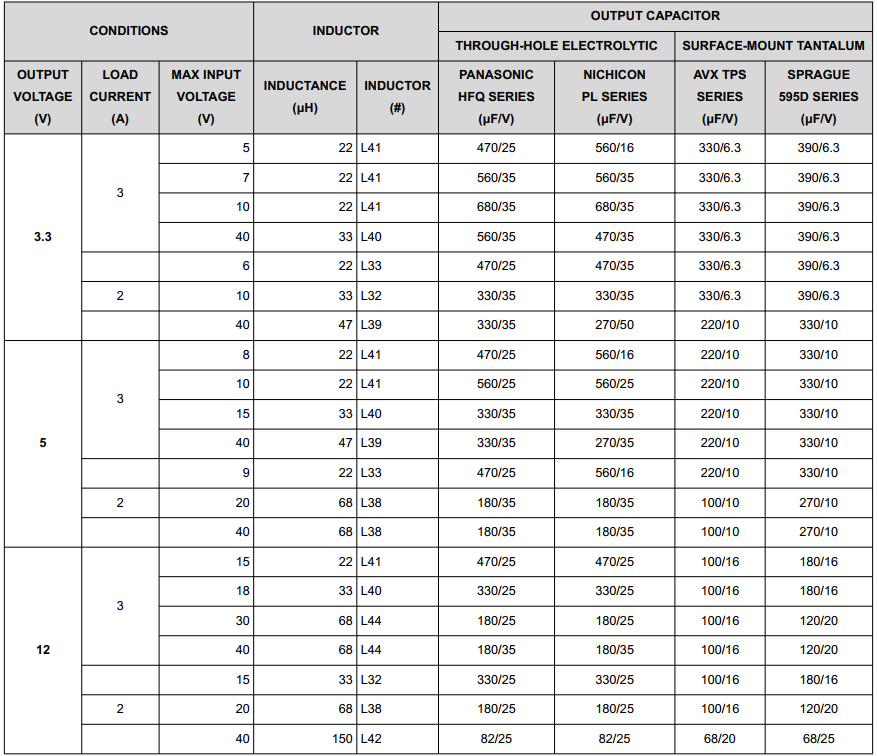
\includegraphics[width=1\textwidth]{pictures/appendix/app_p3_ChooseComponent.png}
                \caption{Cuộn cảm và tụ điện}
                \label{fig:InductorAndCapacitor}
            \end{figure}
        \subsection[Diode cho mạch hạ áp]{Diode cho mạch hạ áp\footnote{Tài liệu tham khảo: \cite{lm2596}, trang 26}}
            \begin{figure}[H]
                \centering
                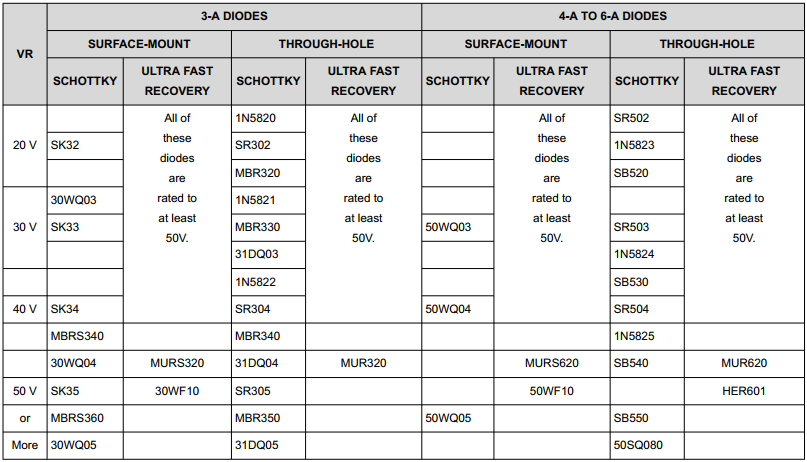
\includegraphics[width=1\textwidth]{pictures/appendix/app_p4_DiodeChoose.png}
                \caption{Diode Schottky 1N5822}
                \label{fig:Diode}
            \end{figure}

    \section{Các linh kiện cơ khí}
        
